% DO NOT COMPILE THIS FILE DIRECTLY!
% This is included by the other .tex files.

%\colorlet{punct}{red!60!black}
%\definecolor{background}{HTML}{EEEEEE}
%\definecolor{delim}{RGB}{20,105,176}
%\colorlet{numb}{magenta!60!black}

\lstdefinelanguage{json}{
    basicstyle=\ttfamily\footnotesize,
    numbers=left,
    numberstyle=\ttfamily\footnotesize,
    stepnumber=1,
    numbersep=8pt,
    showstringspaces=false,
    breaklines=true,
    frame=lines,
    backgroundcolor=\color{background},
    literate=
     *{0}{{{\color{numb}0}}}{1}
      {1}{{{\color{numb}1}}}{1}
      {2}{{{\color{numb}2}}}{1}
      {3}{{{\color{numb}3}}}{1}
      {4}{{{\color{numb}4}}}{1}
      {5}{{{\color{numb}5}}}{1}
      {6}{{{\color{numb}6}}}{1}
      {7}{{{\color{numb}7}}}{1}
      {8}{{{\color{numb}8}}}{1}
      {9}{{{\color{numb}9}}}{1}
      {:}{{{\color{punct}{:}}}}{1}
      {,}{{{\color{punct}{,}}}}{1}
      {\{}{{{\color{delim}{\{}}}}{1}
      {\}}{{{\color{delim}{\}}}}}{1}
      {[}{{{\color{delim}{[}}}}{1}
      {]}{{{\color{delim}{]}}}}{1},
}

\begin{frame}[t,plain]
\titlepage
\end{frame}

\begin{frame}
    \frametitle{MISP - VM}
    \begin{itemize}
    \item Aanmeldgegevens
        \begin{itemize}
            \item MISP admin: admin@admin.test/admin
            \item SSH: misp/Password1234
        \end{itemize}
    \item Beschikbaar op deze locatie (zowel VirtualBox als VMWare):
        \begin{itemize}
                \item \url{https://www.circl.lu/misp-images/latest/}
        \end{itemize}
    \end{itemize}
\end{frame}

\begin{frame}
    \frametitle{MISP - VM}
    \begin{itemize}
    \item Je moet zelf wel nog enkele aanpassingen doen
        \begin{itemize}
            \item sudo -s
            \item cd /var/www/MISP/
            \item sudo pear install INSTALL/dependencies/Console\_CommandLine/package.xml
            \item sudo pear install INSTALL/dependencies/Crypt\_GPG/package.xml
            \item cd /usr/local/src/misp-modules
            \item pip3 install -r REQUIREMENTS
            \item pip3 install .
            \item reboot
        \end{itemize}
    \end{itemize}
\end{frame}

\begin{frame}
    \frametitle{MISP - Algemeen gebruik}
    De planning voor deze training
        \begin{itemize}
            \item Het data model
            \item Bekijken van gegevens
            \item Aanmaken van gegevens
            \item Verschillende vormen van samenwerking
            \item Verdelen van informatie
            \item Exporteren van gegevens
        \end{itemize}
\end{frame}

\begin{frame}
    \frametitle{MISP - Event \newline (de basis bouwsteen van MISP)}
    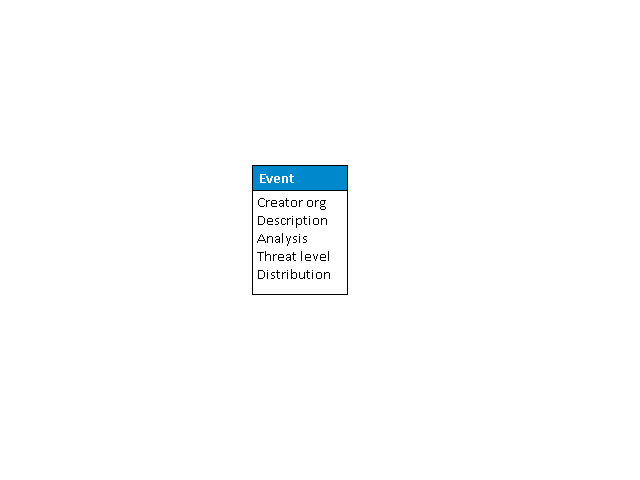
\includegraphics[scale=0.45]{screenshots/datamodel1.png}
\end{frame}

\begin{frame}
    \frametitle{MISP - Event \newline (Attributen, geven een betekenis aan events)}
    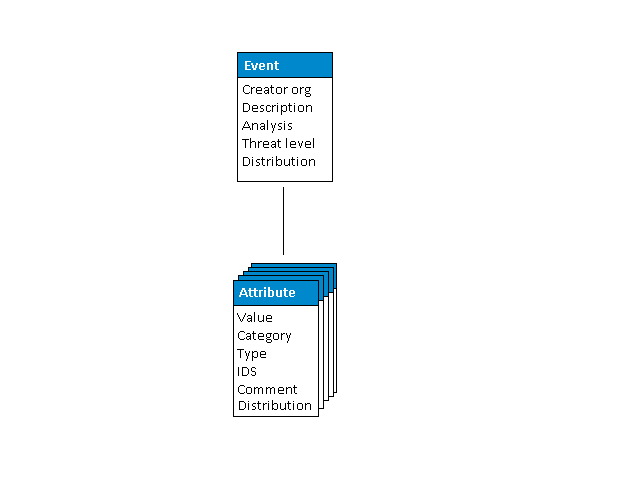
\includegraphics[scale=0.45]{screenshots/datamodel2.png}
\end{frame}

\begin{frame}
    \frametitle{MISP - Event \newline (Correlaties op gelijkaardige attributen)}
    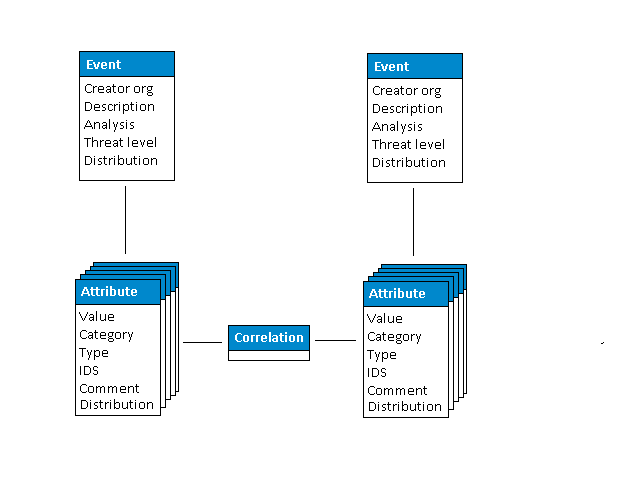
\includegraphics[scale=0.45]{screenshots/datamodel3.png}
\end{frame}

\begin{frame}
    \frametitle{MISP - Event \newline (Voorstellen voor Attributen)}
    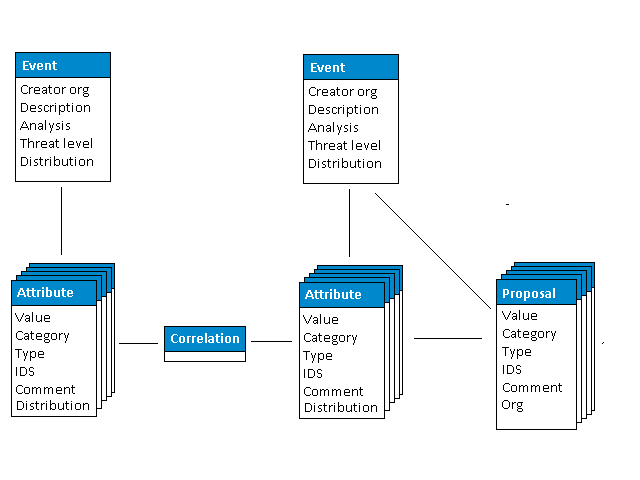
\includegraphics[scale=0.45]{screenshots/datamodel4.png}
\end{frame}

\begin{frame}
    \frametitle{MISP - Event (Tags)}
    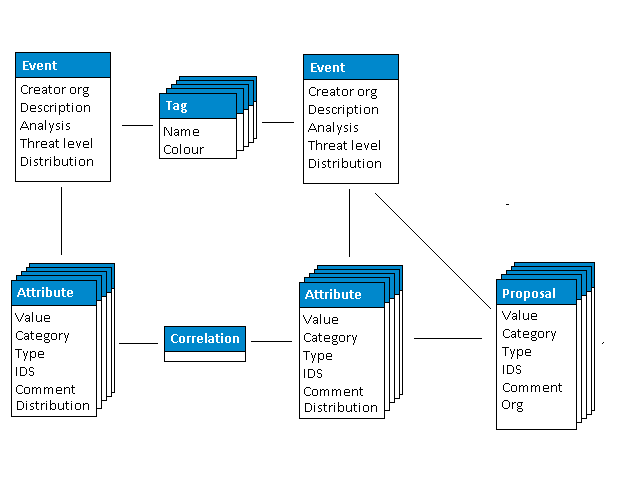
\includegraphics[scale=0.45]{screenshots/datamodel5.png}
\end{frame}

\begin{frame}
    \frametitle{MISP - Event (Discussies)}
    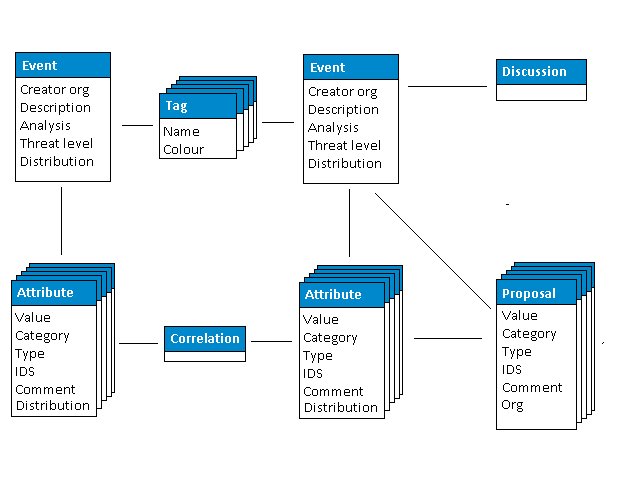
\includegraphics[scale=0.45]{screenshots/datamodel6.png}
\end{frame}

\begin{frame}
    \frametitle{MISP - Event \newline (Taxonomieën en correlaties tussen voorstellen)}
    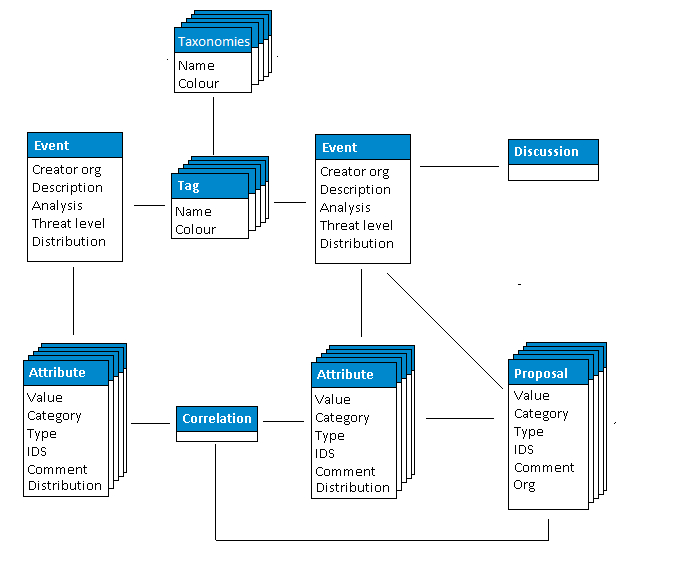
\includegraphics[scale=0.35]{screenshots/datamodel7.png}
\end{frame}

\begin{frame}
    \frametitle{MISP - Event \newline (Het allernieuwste MISP datamodel)}
    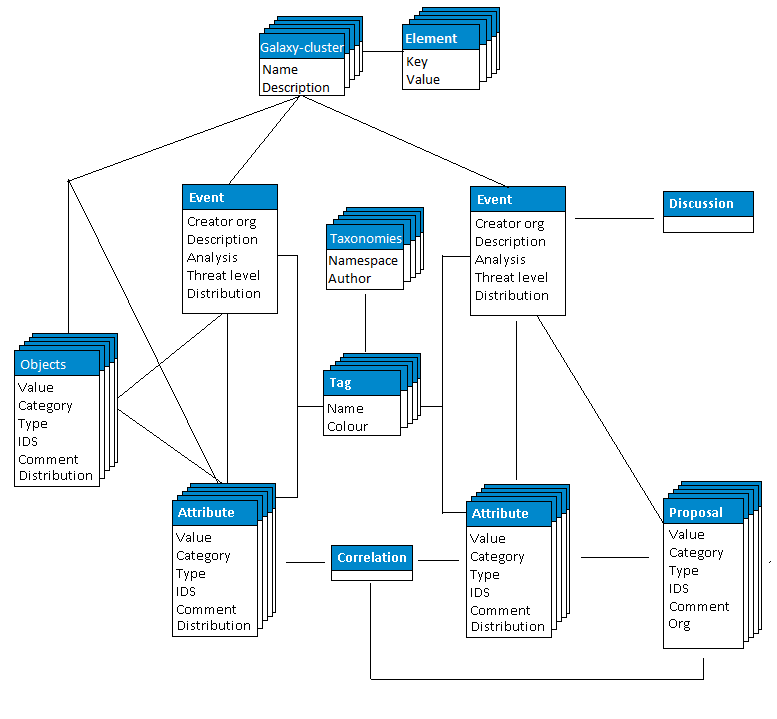
\includegraphics[scale=0.25]{screenshots/datamodel8.png}
\end{frame}

\begin{frame}
    \frametitle{MISP - De lijst van Events Bekijken}
    \begin{itemize}
    \item Lijst van Events
        \begin{itemize}
            \item De context van het event
            \item Tags
            \item Verdelingen
            \item Correlaties
        \end{itemize}
    \item Filters
    \end{itemize}
\end{frame}

\begin{frame}
    \frametitle{MISP - Een Event Bekijken}
    \begin{itemize}
     \item Event scherm
        \begin{itemize}
            \item Context van het event
            \item Attributen
            \begin{itemize}
                \item Verschillende categorieën/types, IDS, Correlaties
            \end{itemize}
            \item Objecten
            \item Galaxies
            \item Voorstellen voor attributen
            \item Discussies
        \end{itemize}
    \item Hulpmiddelen als ondersteuning om te vinden wat je zoekt
    \item Grafieken voor correlatie
    \end{itemize}
\end{frame}

\begin{frame}
    \frametitle{MISP - Verschillende manieren om een event aan te maken en aan te vullen (demo)}
    \begin{itemize}
    \item De belangrijkste hulpmiddelen om een event aan te vullen
        \begin{itemize}
            \item Bijvoegen van attributen / in groep bijvullen van attributen
            \item Bijvoegen van objecten en hoe de templates voor objecten werken
            \item Invoeren via vrije tekst
            \item Importeren
            \item Templates
            \item Bijvoegen van bijlagen / schermafbeeldingen
            \item API
        \end{itemize}
    \end{itemize}
\end{frame}

\begin{frame}
    \frametitle{MISP - Functies beschikbaar tijdens het bijvoegen van gegevens}
    \begin{itemize}
        \item Wat gebeurt er automatisch tijdens het toevoegen van gegevens?
        \begin{itemize}
            \item Automatische correlatie
            \item Aanpassingen van de invoer via validatie en filters (regex)
            \item Tagging / Clusters van Galaxies
        \end{itemize}
        \item De verschillende manieren om gegevens te publiceren
        \begin{itemize}
            \item Publiceren met of zonder e-mail
            \item Publiceren via de API
            \item Publiceren door middel van delegatie
        \end{itemize}
    \end{itemize}
\end{frame}

\begin{frame}
    \frametitle{MISP - Manieren om de gegevens te gebruiken}
    \begin{itemize}
        \item Grafieken voor correlatie
        \item Downloaden van gegevens in verschillende formaten
        \item Voorgemaakte exports
        \item API (later besproken)
        \item Samenwerking met gebruikers (voorstellen, discussies, emails)
    \end{itemize}
\end{frame}

\begin{frame}
    \frametitle{MISP - Synchronisatie uitgelegd (voor de 'niet-admin' training)}
    \begin{itemize}
        \item Het synchronizeren van connecties
        \item Trekken (Pull) of Duwen (Push) model
        \item Vooraf bekijken van een instantie
        \item Filters voor de synchronisatie
        \item De connectie eerst testen
        \item Selectieve keuzes voor synchronisatie
    \end{itemize}
\end{frame}

\begin{frame}
    \frametitle{MISP - Feeds uitgeled (voor de 'niet-admin' training)}
    \begin{itemize}
        \item Types van feeds (MISP, vrije tekst, CSV)
        \item Bijvoegen of aanpassen van feeds
        \item Vooraf bekijken van feeds
        \item Lokale feeds ten opzichte van netwerk feeds
    \end{itemize}
\end{frame}

\begin{frame}
    \frametitle{MISP - Verdeling van informatie uitgelegd}
    \begin{itemize}
        \item Enkel jouw organnisatie
        \item Enkel deze gemeenschap
        \item Aangesloten gemeenschappen
        \item Alle gemeenschappen
        \item Groepen voor delen
    \end{itemize}
\end{frame}

\begin{frame}
    \frametitle{MISP - Verdeling en Topologie}
    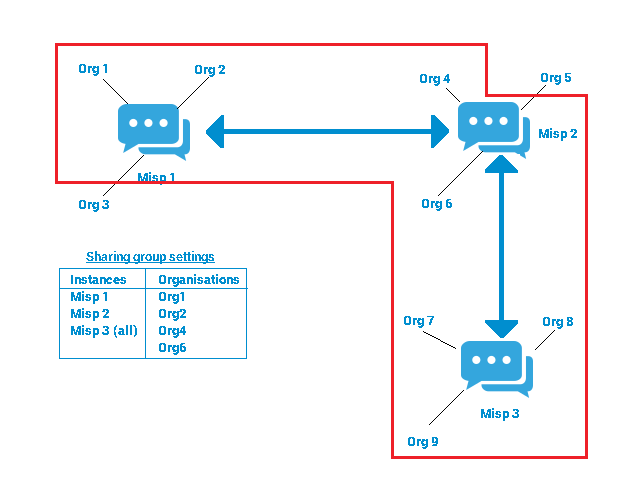
\includegraphics[scale=0.45]{screenshots/sync.png}
\end{frame}

\begin{frame}
    \frametitle{MISP - Exporteren en API}
    \begin{itemize}
        \item Downloaden van een event
        \item Een snelle introductie tot de APIs
        \item Downloaden van zoekresultaten
        \item Voorgemaakte exports
    \end{itemize}
\end{frame}

\begin{frame}
    \frametitle{MISP - Eenvoudige intro tot admin (voor de 'niet-admin' training)}
    \begin{itemize}
        \item Instellingen
        \item Het oplossen van problemen
        \item Ondersteuners (workers)
        \item Logbestanden
    \end{itemize}
\end{frame}
